% Created 2016-03-23 Wed 08:45
\documentclass[11pt]{article}
\usepackage[utf8]{inputenc}
\usepackage{lmodern}
\usepackage[T1]{fontenc}
\usepackage{fixltx2e}
\usepackage{graphicx}
\usepackage{longtable}
\usepackage{float}
\usepackage{wrapfig}
\usepackage{rotating}
\usepackage[normalem]{ulem}
\usepackage{amsmath}
\usepackage{textcomp}
\usepackage{marvosym}
\usepackage{wasysym}
\usepackage{amssymb}
\usepackage{amsmath}
\usepackage[version=3]{mhchem}
\usepackage[numbers,super,sort&compress]{natbib}
\usepackage{natmove}
\usepackage{url}
\usepackage{minted}
\usepackage{underscore}
\usepackage[linktocpage,pdfstartview=FitH,colorlinks,
linkcolor=blue,anchorcolor=blue,
citecolor=blue,filecolor=blue,menucolor=blue,urlcolor=blue]{hyperref}
\usepackage{attachfile}
\usepackage[left=1in, right=1in, top=1in, bottom=1in, nohead]{geometry}
\geometry{margin=1.0in}
\usepackage{amsmath}
\usepackage{siunitx}
\usepackage{graphicx}
\usepackage{epstopdf}
\usepackage{fancyhdr}
\usepackage{hyperref}
\usepackage[labelfont=bf]{caption}
\usepackage{setspace}
\usepackage{sectsty}
\subsectionfont{\rm}
\setlength{\headheight}{5.2pt}
\setlength{\headsep}{14pt}
\def\dbar{{\mathchar'26\mkern-12mu d}}
\pagestyle{fancy}
\fancyhf{}
\renewcommand{\headrulewidth}{0.5pt}
\renewcommand{\footrulewidth}{0.5pt}
\lfoot{\today}
\cfoot{\copyright\ 2016 W.\ F.\ Schneider}
\rfoot{\thepage}
\rhead{\bf{ND CBE 20255}}
\lhead{\bf{Exam 2}}
\chead{\bf{Spring 2016}}
\setcounter{secnumdepth}{3}
\author{William F. Schneider}
\date{\today}
\title{CBE 60553 Outline}
\begin{document}

\begin{options}
\end{options}

\
\vspace{2cm}
\begin{figure}[h]
\centering

\includegraphics[width=0.4\textwidth]{./centered-2c-NDmark.pdf}
\end{figure}
\begin{center}
{\LARGE\bf Introduction to Chemical Engineering\\(CBE 20255)}
\vspace{0.5cm}

{\Large Prof. William F.\ Schneider}
\end{center}
\vspace{2cm}
\noindent\large{{\bf NAME (PRINT):}}\_\_\_\_\_\_\_\_\_\_\_\_\_\_\_\_\_\_\_\_\_\_\_\_\_\_\_\_\_\_\_\_\_\_\_\_\_\_

\vspace{1cm}
\begin{spacing}{1.2}
\begin{tabular}{|p{5.5in}|}
\hline
{\em AS A MEMBER OF THE NOTRE DAME COMMUNITY, I WILL NOT PARTICIPATE IN OR
TOLERATE ACADEMIC DISHONESTY } \\
\hline
\end{tabular}
\end{spacing}
\vspace{1.5cm}

\noindent\large{{\bf SIGNED:}} \_\_\_\_\_\_\_\_\_\_\_\_\_\_\_\_\_\_\_\_\_\_\_\_\_\_\_\_\_\_\_\_\_\_\_\_\_\_\_\_\_\_\_\_

\vspace{1cm}
\noindent{\bf PLEASE SHOW YOUR WORK.  CLEARLY DEMONSTRATE YOUR SOLUTION PROCEDURE
AND STATE ANY ASSUMPTIONS YOU MAKE.  WRITE YOUR SOLUTIONS IN THE SPACE
PROVIDED.  BLANK PAGES ARE INCLUDED TO PROVIDE MORE ROOM FOR YOUR
WORK.  ASK THE PROCTOR IF YOU NEED ADDITIONAL SCRATCH PAPER.}
\newpage


\section{Maintaining My Equilibrium (50 pts)}
\label{sec-1}
The equilibrium between the liquid and vapor phases of two fluids (let's call them A and B) is given by the following \emph{Txy} diagram at a fixed pressure of 1 atmosphere:

\begin{center}
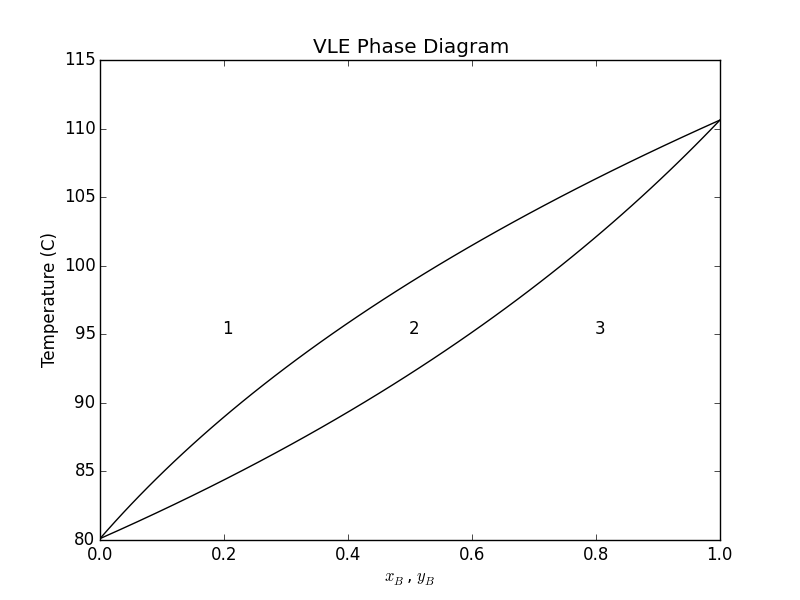
\includegraphics[width=0.75\textwidth]{./TemperatureVLE.png}
\end{center}

\subsection{(5 pts) What is the normal boiling point of the B component?}
\label{sec-1-1}
\vspace{2cm}
\subsection{(15 pts) Complete the table below.  For each point, indicate which phase(s) are present and what their compositions are.}
\label{sec-1-2}

\begin{center}
\begin{tabular}{lcc}
\hline
Point & Liquid phase composition & Vapor phase composition\\
\hline
 &  & \\
1 &  & \\
 &  & \\
 &  & \\
2 &  & \\
 &  & \\
 &  & \\
3 &  & \\
 &  & \\
\hline
\end{tabular}
\end{center}
\newpage
\subsection{(5 pts) Which (if any) of the points is superheated?  By how many Celsius degrees?}
\label{sec-1-3}
\vspace{2cm}
\subsection{(5 pts) What is the \textbf{bubble point} temperature when the liquid phase is a 50:50 molar mixture of the two components?}
\label{sec-1-4}
\vspace{2cm}
\subsection{(5 pts) What is the \textbf{dew point} temperature when the vapor phase is a 50:50 molar mixture of the two components?}
\label{sec-1-5}
\vspace{2cm}
\subsection{(10 pts) Component A has an enthalpy of vaporization of \SI{83.1}{\joule\per\mole}. Estimate the temperature at which pure liquid A is in equilibrium with vapor A at 1 atmosphere gauge pressure.}
\label{sec-1-6}
\newpage
\subsection{(5 pts) Suppose components A and B were not miscible; that is, when mixed, they made two distinct liquid phases. Is it possible for these two liquids to be in equilibrium with a third vapor phase?  If so, how many and which intensive variables could be specified at the conditions at which these three co-exist?  Explain your answer.}
\label{sec-1-7}
\newpage
\section{Partial oxidation (30 pts)}
\label{sec-2}
Ethylene oxide (\ce{C2H4O}) is produced by the partial oxidation of ethylene (\ce{C2H4}) by \ce{O2}.  The complete oxidation of ethylene oxide to \ce{CO2} and \ce{H2O} is an undesirable side reaction.
\\ \\
Ethylene oxide is produced in a recycle reactor.  The reactor feed contains 3 moles \ce{C2H4} per mole \ce{O2}. The single pass ethylene conversion is 20\%, and for every 100 moles of ethylene consumed, 90 moles of ethylene oxide are produced.  The reactor effluent is separated into an ethylene oxide stream, which is sold, a combined \ce{CO2}/\ce{H2O} stream, which is discarded, and an ethylene and oxygen stream, which is recycled.
\subsection{(5 pts) Write balanced equations for the partial and complete oxidations of ethylene.}
\label{sec-2-1}
\vspace{6cm}
\subsection{(5 pts) Make a sketch of this process, labeling all flows and compositions and identifying unknowns by drawing boxes around them. Assume an inlet basis into the reactor of 100 mol/s.}
\label{sec-2-2}
\newpage
\subsection{(10 pts) What is the composition and molar flow rate of the ethylene/\ce{O2} recycle stream?}
\label{sec-2-3}
\vspace{10cm}
\subsection{(10 pts) What is the required composition and molar flow rate of the fresh feed?}
\label{sec-2-4}
\newpage
\section{Oh Henry! (20 pts)}
\label{sec-3}
Ionic liquids (ILs) are an unusual class of liquids that have negligible vapor pressure. Amongst other interesting properties is their ability to selectively absorb  gases.  For instances, the Henry's Law constants of \ce{CO2} and \ce{CH4} in a representative IL at ambient temperature are reported by Anthony \textit{et al.}, \emph{J. Phys. Chem. B} \textbf{2002}, to be 53 and 1700 bar, respectively.
\\ \\
Your job is to reduce the \ce{CO2} concentration in a 50/50 \ce{CO2}/\ce{CH4} gas mixture by 90\%.  The gas mixture is sent into a stripper column at ambient temperature and 100~bar total pressure in parallel with a stream of pure IL.  Exiting the stripper is a gas mixture of the desired composition and the same temperature and pressure, and a liquid IL stream containing the dissolved gases.
\subsection{(5 pts) What is the composition of the exiting gas phase?}
\label{sec-3-1}
\vspace{3cm}
\subsection{(5 pts) What is the composition of the exiting liquid phase?}
\label{sec-3-2}
\vspace{4cm}
\subsection{(10 pts) What is the ratio of the inlet molar flow rate of gas mixture to IL?}
\label{sec-3-3}
% Emacs 25.0.50.1 (Org mode 8.2.10)
\end{document}